% Section: setup (\input from main.tex)
\section{Experimental Setup and Methodology}
\label{sec:setup}

\subsection{Code organization}

The project is a single \texttt{Makefile} build (C++17, \texttt{-O2},
\texttt{-pthread}) with header-only implementations, separate correctness
tests, and benchmark drivers:

\begin{center}
\small
\begin{tabularx}{\linewidth}{>{\ttfamily}l X}
\toprule
\textrm{\textbf{File}} & \textbf{Content} \\
\midrule
src/graph.hpp      & CSR road graph with integer costs, admissible straight-line bound, CSV loader \\
src/seq\_astar.hpp & Part 1: Dijkstra (test oracle), generic A*, Euclidean / uncertain / dynamic / ALT / costly heuristics, \NAMOA \\
src/clist.hpp      & Part 2: \texttt{CoarseList}, \texttt{FineList}, \texttt{OptimisticList}, \texttt{LazyList}; \texttt{MutexLock}, \texttt{TTASLock}, \texttt{BackoffLock}; \texttt{removeMin} \\
src/par\_astar.hpp & Part 3: parallel A* over a shared open list (any list, or a locked heap); \HDA{} with optional $f$-window \\
src/route.cpp      & command-line route planner (GeoJSON output) \\
tests/             & \texttt{test\_seq}, \texttt{test\_clist}, \texttt{test\_par} (also built with ThreadSanitizer) \\
bench/             & \texttt{bench\_seq}, \texttt{bench\_clist}, \texttt{bench\_astar} \\
scripts/           & \texttt{build\_graph.py} (OSM $\rightarrow$ graph), figure and table scripts \\
run\_all.sh, run\_mac.sh & build, run all tests, then the full benchmark sweep on one platform \\
\bottomrule
\end{tabularx}
\end{center}

All benchmarks write CSV files named \texttt{results/<experiment>\_<platform>.csv};
all tables and figures in this report are regenerated from those files.

\subsection{Road network}

The lecturer's notebook downloads the drive network of the whole city with
OSMnx. From our networks the OSMnx services were not usable: Nominatim, which
turns the place name into a boundary, was blocked, and all public Overpass
servers were overloaded (HTTP 429, 502, 504). We therefore built the graph
from Geofabrik's OpenStreetMap extract of Vietnam (\texttt{vietnam-latest.osm.pbf},
332\,MB, \copyright{} OpenStreetMap contributors, ODbL) with
\texttt{scripts/pbf\_to\_graph.py}:

\begin{itemize}[nosep]
  \item The bounding box covers urban Ho Chi Minh City (latitude 10.65--10.92,
        longitude 106.55--106.88): Districts 1--12, Binh Thanh, Phu Nhuan, Go
        Vap, Tan Binh, Tan Phu, Binh Tan, Thu Duc City, Nha Be and the urban
        parts of Binh Chanh and Hoc Mon. It contains both end points of the
        lecturer's example.
  \item It keeps every road a motorbike may use (motorway to residential
        roads, links, living streets and service roads except parking aisles
        and driveways; \texttt{access=no/private} removed) and honours one-way
        tags and roundabouts.
  \item Like OSMnx, it simplifies the graph: nodes are kept only where roads
        end, meet, or leave the box, and an edge gets the summed length of the
        road segments it replaces.
  \item It keeps the largest strongly connected component, so every pair of
        nodes has a route.
\end{itemize}

The result has \textbf{203\,396 nodes and 455\,837 directed edges}
(Figure~\ref{fig:map}). The lecturer's example, from Thu Thiem
(10.768856, 106.725019) to Thu Duc (10.839613, 106.845798), is a 19.1\,km
route that A* with ALT finds after 5\,058 expansions, against 154\,943 for
Dijkstra. Part~2 does not use the graph. During development we also used a
small extract of the city centre (33\,718 nodes); \texttt{osm-astar-fixed.ipynb}
can still run on it.

Every edge carries three integer costs: \emph{length} in millimetres,
free-flow \emph{time} in milliseconds (from \texttt{maxspeed}, or a per-class
default of 10--60\,km/h), and rush-hour \emph{congested time} (free-flow time
multiplied by 1.0--2.6 depending on the road class, because main roads are the
most congested). We use integers on purpose: sequential and parallel results
can then be compared for exact equality, with no floating-point tolerance.
The time-dependent model of Section~\ref{sec:seq-td} uses the lecturer's speed
profile instead.

\begin{figure}[H]
\centering
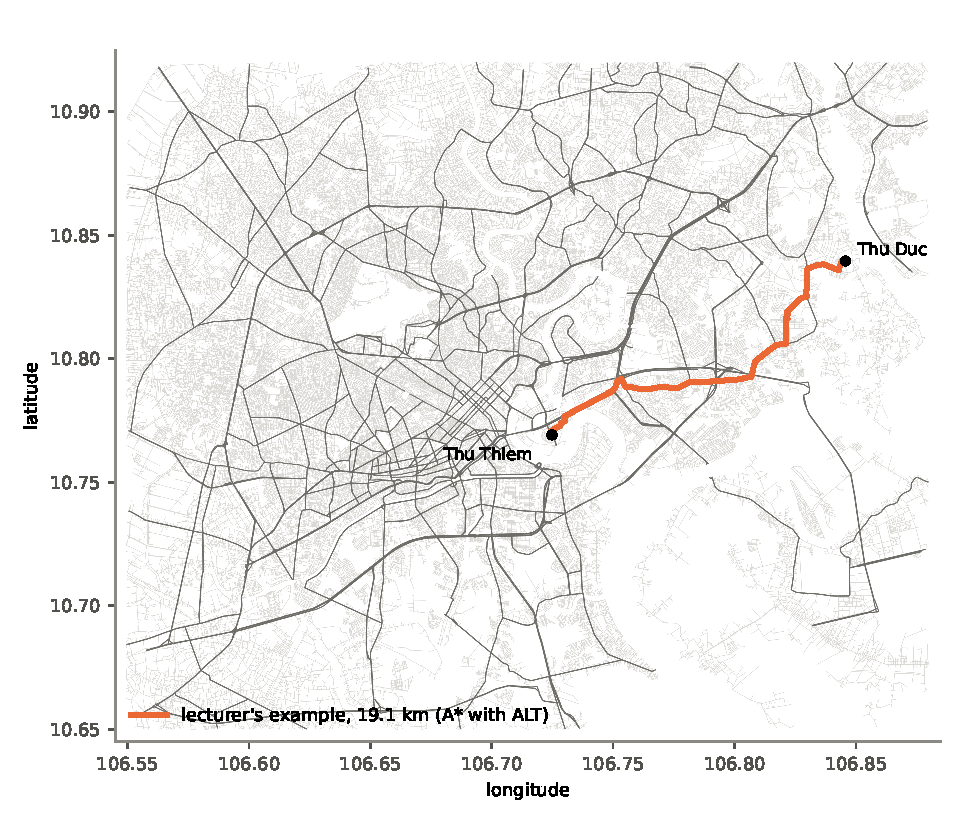
\includegraphics[width=0.8\linewidth]{figures/fig1_map.pdf}
\caption{The road graph of urban Ho Chi Minh City (major roads darker) and the
lecturer's example query. Every algorithm in this report returns this route
(\texttt{./bin/route 10.768856 106.725019 10.839613 106.845798 --algo alt --data data\_city}).}
\label{fig:map}
\end{figure}

\subsection{Parameters and measurement}

\begin{center}
\small
\begin{tabularx}{\linewidth}{l Y Y}
\toprule
\textbf{Part} & \textbf{Swept parameters} & \textbf{Fixed amount of work} \\
\midrule
1 Sequential A* & heuristic, metric (length, time), error $\varepsilon\in\{0.1,0.3,0.5,1,2\}$, departure time & 200 random queries with straight-line distance $>1$\,km; 40 bi-objective queries (0.5--4.5\,km); 40 simulated trips ($\ge 3.5$\,km) \\
2 Lists  & list $\times$ lock (12 variants), threads $\in\{1,2,4,8,16\}$, workload mix & key range 1\,000, half pre-filled; each run lasts 0.4\,s \\
3 Parallel A* & version (12 parallel + sequential), heuristic (4), threads $\in\{1,2,4,8,16\}$ & 20 long queries ($>5$\,km, about 99\,000 Dijkstra expansions each) \\
\bottomrule
\end{tabularx}
\end{center}

Part~1 reports the mean time per query. Part~2 reports throughput in million
operations per second; Part~3 reports the wall time to answer all 20 queries
one after another, so thread creation and joining is included once per query.
Each Part~2 and Part~3 configuration is repeated 3 times and we report the
\textbf{median}. Time is measured with \texttt{std::chrono::steady\_clock}.
Part~2 used threads $\in\{1,2,4,8,16\}$ on Platform~A, $\{1,2,4,8\}$ on
Platforms~B and~C, and $\{1,2,4,8,10,16,20,32\}$ on Platform~D; Part~3 used up to twice the hardware threads (capped at 32 on D):
$\{1,\dots,16\}$ on A, $\{1,2,4,8\}$ on B, $\{1,2,4\}$ on C, and $\{1,2,4,8,10,16,20,32\}$ on D. Shaded regions in the figures mark thread counts that exceed
the hardware threads available. An extended sweep (\texttt{run\_ext.sh}) on Platform~D additionally measures 5--7 repetition spread, persistent \texttt{ThreadPool} vs.\ per-query spawning, physical-core-first pinning, key ranges up to 50\,000, \texttt{TTASLock} in Part~3, the \texttt{TIME} metric, and \HDA{} $f$-window tuning.

Solution \emph{quality} is measured as cost divided by the exact optimum from
Dijkstra. All exact algorithms (every parallel version included) reach a ratio
of exactly 1.000000 in every run, so quality only differs in the deliberately
inexact variants of Sections~\ref{sec:seq-dyn} and~\ref{sec:seq-td}.

\subsection{Platforms}

The assignment requires at least as many platforms as group members.
Table~\ref{tab:platforms} lists them.

\begin{table}[H]
\centering
\scriptsize
\caption{Shared-memory platforms used in the study.}
\label{tab:platforms}
\begin{tabularx}{\linewidth}{l YYYY}
\toprule
 & \textbf{Platform A} & \textbf{Platform B} & \textbf{Platform C} & \textbf{Platform D} \\
\midrule
Machine       & MacBook Pro (Apple M5), native & Linux VM on the same MacBook Pro & Cloud virtual machine & Workstation (bare-metal) \\
CPU           & Apple M5, 4P + 6E cores & Apple M5 (4 vCPUs) & Intel Xeon @ 2.10\,GHz & Intel Xeon W-2255 @ 3.70\,GHz \\
Cores / HW threads & 10 / 10 & 4 / 4 & 2 / 2 & 10 / 20 (SMT) \\
Memory        & 16\,GiB & 4\,GiB & 8\,GiB & 61\,GiB \\
OS            & macOS 27.2 & Ubuntu 22.04 (aarch64) & Ubuntu 24.04 (x86-64) & Ubuntu (x86-64, Linux 7.0) \\
Compiler / C++ library & Apple Clang 21.0, libc++ & GCC 11.4, libstdc++ & GCC 13.3, libstdc++ & GCC 15.2, libstdc++ \\
Memory model  & ARMv8 (weak) & ARMv8 (weak) & x86-64 TSO & x86-64 TSO \\
\bottomrule
\end{tabularx}
\end{table}

The platforms differ in instruction set and memory model, operating system and
scheduler, C++ library, and core count. Two of them are ARM machines, so the
acquire/release orderings of our lock-free list traversals are exercised on a
weak memory model and not only on x86. Platform~A is heterogeneous (only
4 of its 10 cores are performance cores), whereas Platform~D provides 10 uniform
physical cores (20 hardware threads with SMT) without hypervisor scheduling.
One caveat applies to Platform~A: random query pairs are drawn with
\texttt{std::\allowbreak uniform\_int\_\allowbreak distribution}, whose algorithm differs between libc++
and libstdc++. Platform~A therefore answers a different (statistically
equivalent) query set from B, C, and D (which share identical libstdc++ queries). Speed-ups are always computed against the
sequential run on the same platform and the same queries, so they remain
comparable.
